\subsection{UC6 - Personalizzazione della visualizzazione}
\begin{figure}[h]
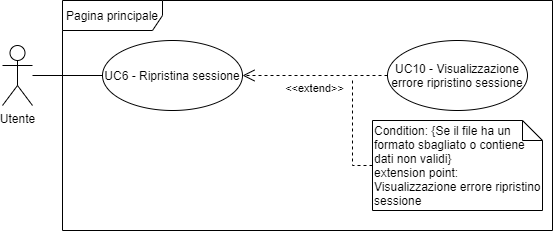
\includegraphics[width=\linewidth]{Section/Images/UC6.png}
\centering
\caption{UC6 - Personalizzazione della visualizzazione scelta}
\end{figure}
\begin{itemize}
	\item \textbf{Attore primario}: Utente;
	
	\item \textbf{Precondizioni}: L'utente ha scelto il grafico tra quelli a disposizione nel sistema [UC5];
	
	\item \textbf{Postcondizioni}: Il grafico viene aggiornato con le personalizzazioni impostate dall'utente;
	
	\item \textbf{Scenario principale}: L’utente sceglie come impostare le opzioni di personalizzazione del grafico. Verranno applicati, per ciascun campo, dei valori di default che l'utente può decidere di modificare o meno. In caso fosse stato precedentemente caricato un file di ripristino sessione [UC1.2] i valori di default iniziali diventerebbero quindi quelli specificati in questo file, lasciando comunque all'utente la possibilità di modificarli;
	
	\item \textbf{Generalizzazioni}: L'utente imposta i parametri di personalizzazione della visualizzazione scelta:
	\begin{enumerate}[(a)]
	\item Personalizzazione \textit{Scatter Plot Matrix} [UC6.1];
	\item Personalizzazione \textit{Heat Map} [UC6.2];
	\item Personalizzazione \textit{Force Field} [UC6.3];
	\item Personalizzazione \textit{Proiezione Lineare Multi Asse} [UC6.4].
	\end{enumerate}
		
\end{itemize}


